\documentclass[10pt]{article}

% basic packages
\usepackage[margin=1in]{geometry}
\usepackage[pdftex]{graphicx}
\usepackage{amsmath,amssymb,amsthm}
\usepackage{custom}
\usepackage{lipsum}
\usepackage{tikz}

% page formatting
\usepackage{fancyhdr}
\pagestyle{fancy}

\renewcommand{\sectionmark}[1]{\markright{\textsf{\arabic{section}. #1}}}
\renewcommand{\subsectionmark}[1]{}
\newcommand{\m}[1]{$#1$}
\lhead{\scriptsize\textbf{\thepage}\ \ \nouppercase{\rightmark}}
\chead{}
\rhead{\normalfont MAP2302 - Spring 2026}
\lfoot{}
\cfoot{}
\rfoot{}
\setlength{\headheight}{14pt}

\linespread{1.03}
\setlength{\parindent}{0pt}
\setlength{\parskip}{6pt}
\setcounter{secnumdepth}{3}
\setcounter{tocdepth}{3}

% annotation spacing helper — adjust the default length as needed
\newcommand{\annotspace}[1][3.5cm]{\vspace{#1}}

\begin{document}

% ============================================================
% TITLE PAGE
% ============================================================
\thispagestyle{empty}
\vspace*{3cm}

\begin{center}
    {\fontsize{13}{13}\selectfont\sffamily Palm Beach State College \quad\textbullet\quad Spring 2026}
    \vskip 20pt
    \rule{0.6\linewidth}{0.4pt}
    \vskip 20pt
    {\fontsize{28}{28}\selectfont\bfseries\sffamily Unit 02 Study Notes}
    \vskip 12pt
    {\fontsize{16}{16}\selectfont\rmfamily MAP2302 \quad Differential Equations}
    \vskip 20pt
    \rule{0.6\linewidth}{0.4pt}
    \vskip 24pt
    {\fontsize{15}{15}\selectfont\rmfamily Aspen J.\ Johnson}
    \vskip 6pt
    {\fontsize{11}{11}\selectfont\ttfamily aspen.johnson@pbsc.edu}
    \vskip 30pt
    {\fontsize{11}{11}\selectfont\rmfamily
        Instructor: Professor Tamara Johns\\[4pt]
        Examination: Friday, March 6\textsuperscript{th}, 2026
    }
\end{center}

\vfill

\begin{center}
{\small\itshape
Topics covered: Higher-Order Linear ODEs $\cdot$ Reduction of Order $\cdot$
Constant-Coefficient Equations $\cdot$ Undetermined Coefficients (Superposition \& Annihilator)}
\end{center}
\newpage




% ============================================================
% TABLE OF CONTENTS
% ============================================================
\microtoc

% ============================================================
% APPENDIX — QUICK REFERENCE
% ============================================================
\newpage
\section*{Appendix: Quick Reference}
\addcontentsline{toc}{section}{Appendix: Quick Reference}

% ── A.1  Integration by Parts Shortcuts ─────────────────────
\subsection*{A.1 \quad Integration by Parts Shortcuts}
\addcontentsline{toc}{subsection}{A.1 Integration by Parts Shortcuts}

Recall the IBP formula: \m{\displaystyle\int u\,dv = uv - \int v\,du}.
For repeated application use the \textbf{tabular (tic-tac-toe) method}:
alternate signs \m{+,-,+,-,\ldots}, differentiate the left column to zero,
integrate the right column, then multiply diagonally.

\medskip
\renewcommand{\arraystretch}{1.6}
\begin{center}
\begin{tabular}{lll}
\hline
\textbf{Integral} & \textbf{Result} & \textbf{Notes} \\
\hline
\m{\displaystyle\int x e^{ax}\,dx}
    & \m{\dfrac{e^{ax}}{a}\!\left(x - \dfrac{1}{a}\right) + C}
    & \m{u=x,\; dv=e^{ax}dx} \\

\m{\displaystyle\int x^2 e^{ax}\,dx}
    & \m{\dfrac{e^{ax}}{a}\!\left(x^2 - \dfrac{2x}{a} + \dfrac{2}{a^2}\right) + C}
    & tabular method \\

\m{\displaystyle\int x e^{ax}\cos(bx)\,dx}
    & use tabular twice
    & cycles after 2 steps \\

\m{\displaystyle\int e^{ax}\cos(bx)\,dx}
    & \m{\dfrac{e^{ax}(a\cos bx + b\sin bx)}{a^2+b^2} + C}
    & IBP twice, solve for \m{I} \\

\m{\displaystyle\int e^{ax}\sin(bx)\,dx}
    & \m{\dfrac{e^{ax}(a\sin bx - b\cos bx)}{a^2+b^2} + C}
    & IBP twice, solve for \m{I} \\

\m{\displaystyle\int x\cos(bx)\,dx}
    & \m{\dfrac{\cos(bx)}{b^2} + \dfrac{x\sin(bx)}{b} + C}
    & \m{u=x,\; dv=\cos(bx)dx} \\

\m{\displaystyle\int x\sin(bx)\,dx}
    & \m{\dfrac{\sin(bx)}{b^2} - \dfrac{x\cos(bx)}{b} + C}
    & \m{u=x,\; dv=\sin(bx)dx} \\

\m{\displaystyle\int x^n e^{ax}\,dx}
    & \m{\dfrac{x^n e^{ax}}{a} - \dfrac{n}{a}\displaystyle\int x^{n-1}e^{ax}\,dx}
    & reduction formula \\
\hline
\end{tabular}
\end{center}

\bigskip

% ── A.2  Trigonometric Identities ───────────────────────────
\subsection*{A.2 \quad Trigonometric Identities}
\addcontentsline{toc}{subsection}{A.2 Trigonometric Identities}

\subsubsection*{Reciprocal and Quotient Identities}
\[
\csc x = \frac{1}{\sin x}, \qquad
\sec x = \frac{1}{\cos x}, \qquad
\cot x = \frac{1}{\tan x} = \frac{\cos x}{\sin x}, \qquad
\tan x = \frac{\sin x}{\cos x}.
\]

\subsubsection*{Pythagorean Identities}
\[
\sin^2 x + \cos^2 x = 1, \qquad
1 + \tan^2 x = \sec^2 x, \qquad
1 + \cot^2 x = \csc^2 x.
\]

\subsubsection*{Double-Angle Identities}
\[
\sin(2x) = 2\sin x\cos x, \qquad
\cos(2x) = \cos^2 x - \sin^2 x = 1 - 2\sin^2 x = 2\cos^2 x - 1.
\]

\subsubsection*{Power-Reduction Identities}
\[
\sin^2 x = \frac{1 - \cos(2x)}{2}, \qquad
\cos^2 x = \frac{1 + \cos(2x)}{2}.
\]

\bigskip

% ── A.3  Unit Circle and Domain Restrictions ─────────────────
\subsection*{A.3 \quad Unit Circle and Domain Restrictions}
\addcontentsline{toc}{subsection}{A.3 Unit Circle and Domain Restrictions}

\begin{center}
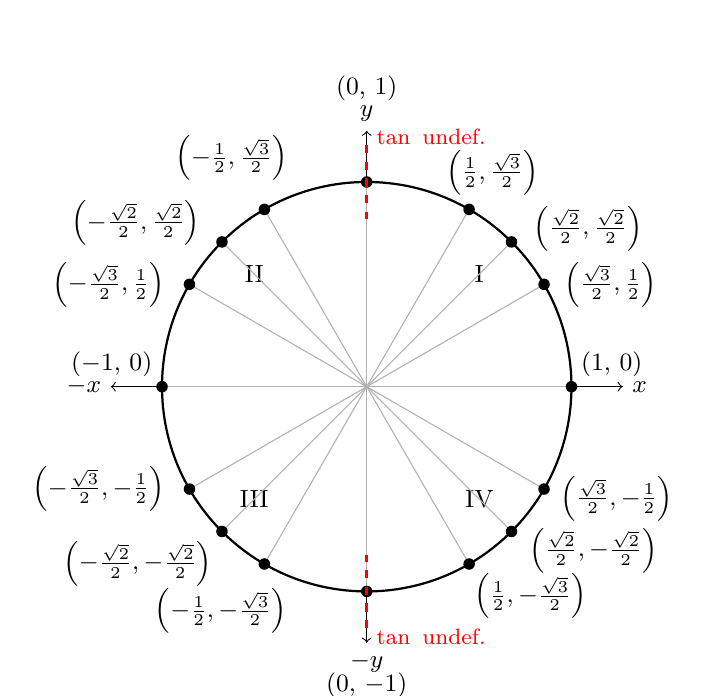
\begin{tikzpicture}[scale=2.6, font=\small]

  % axes
  \draw[->] (-1.25,0) -- (1.25,0) node[right] {\m{x}};
  \draw[->] (1.25,0) -- (-1.25,0) node[left] {\m{-x} };

  \draw[->] (0,1.25) -- (0,-1.25) node[below] {\m{-y}};
  \draw[->] (0,-1.25) -- (0,1.25) node[above] {\m{y}};

  % unit circle
  \draw[thick] (0,0) circle(1);

  % quadrant labels
  \node at ( 0.55, 0.55) {\small I};
  \node at (-0.55, 0.55) {\small II};
  \node at (-0.55,-0.55) {\small III};
  \node at ( 0.55,-0.55) {\small IV};

  % ---- standard angles: (angle, x-coord label offset, y-coord label offset) ----
  \foreach \angle/\cx/\cy/\lab in {
      0    / 0.08 / 0.10 / {0},
      30   / 0.10 / 0.10 / {\pi/6},
      45   / 0.08 / 0.10 / {\pi/4},
      60   / 0.04 / 0.12 / {\pi/3},
      90   / 0.00 / 0.12 / {\pi/2},
      120  / 0.00 / 0.12 / {2\pi/3},
      135  / 0.00 / 0.10 / {3\pi/4},
      150  / 0.00 / 0.10 / {5\pi/6},
      180  / 0.00 / 0.10 / {\pi},
      210  / 0.00 / 0.00 / {7\pi/6},
      225  / 0.00 / 0.00 / {5\pi/4},
      240  / 0.00 / 0.00 / {4\pi/3},
      270  / 0.00 / 0.00 / {3\pi/2},
      300  / 0.00 / 0.00 / {5\pi/3},
      315  / 0.00 / 0.00 / {7\pi/4},
      330  / 0.00 / 0.00 / {11\pi/6}
  }{
    \draw[gray!60, thin] (0,0) -- (\angle:1);
    \fill (\angle:1) circle(0.8pt);
  }

  % ---- labelled points (angle : cos, sin) ----
  \node[above right] at ( 0:1)   {\m{(1,\,0)}};
  \node[above right] at ( 20:1)   {\m{\!\left(\tfrac{\sqrt3}{2},\tfrac{1}{2}\right)}}; %Angle is 30, but moving them down for visibility purposes
  \node[above right] at ( 38:1)   {\m{\!\left(\tfrac{\sqrt2}{2},\tfrac{\sqrt2}{2}\right)}};
  \node[above left]  at ( 45:1.255)   {\m{\!\left(\tfrac{1}{2},\tfrac{\sqrt3}{2}\right)}};
  \node[above]       at ( 90:1.35)   {\m{(0,\,1)}};
  \node[above right] at (135:1.356)   {\m{\!\left(-\tfrac{1}{2},\tfrac{\sqrt3}{2}\right)}};
  \node[above left]  at (140:1)   {\m{\!\left(-\tfrac{\sqrt2}{2},\tfrac{\sqrt2}{2}\right)}};
  \node[above left]  at (160:1)   {\m{\!\left(-\tfrac{\sqrt3}{2},\tfrac{1}{2}\right)}};
  \node[above left]  at (180:1)   {\m{(-1,\,0)}};
  \node[below left]  at (200:1)   {\m{\!\left(-\tfrac{\sqrt3}{2},-\tfrac{1}{2}\right)}};
  \node[below left]  at (225:1)   {\m{\!\left(-\tfrac{\sqrt2}{2},-\tfrac{\sqrt2}{2}\right)}};
  \node[below left]  at (250:1)   {\m{\!\left(-\tfrac{1}{2},-\tfrac{\sqrt3}{2}\right)}};
  \node[below]       at (270:1.35)   {\m{(0,\,-1)}};
  \node[below right] at (300:1)   {\m{\!\left(\tfrac{1}{2},-\tfrac{\sqrt3}{2}\right)}};
  \node[below right] at (320:1)   {\m{\!\left(\tfrac{\sqrt2}{2},-\tfrac{\sqrt2}{2}\right)}};
  \node[below right] at (337:1)   {\m{\!\left(\tfrac{\sqrt3}{2},-\tfrac{1}{2}\right)}};

  % ---- tan undefined markers ----
  \draw[red, very thick, dashed]
      (90:1.18)  -- (90:0.82)
      (270:1.18) -- (270:0.82);
  \node[red, right, font=\footnotesize] at (90:1.22)
      {\m{\tan\text{ undef.}}};
  \node[red, right, font=\footnotesize] at (270:1.22)
      {\m{\tan\text{ undef.}}};

\end{tikzpicture}
\end{center}

\medskip

\noindent\textbf{Why \m{\tan x} causes problems at \m{x = \pm\pi/2}.}\quad
Since \m{\tan x = \sin x / \cos x}, the function is undefined wherever \m{\cos x = 0}, namely at
\m{x = \pm\tfrac{\pi}{2},\, \pm\tfrac{3\pi}{2}, \ldots} On the unit circle these correspond to the
points \m{(0, 1)} and \m{(0, -1)} where the \m{x}-coordinate (i.e.\ \m{\cos x}) is zero.

\medskip

For an ODE such as \m{y'' + (\tan x)\,y = e^x}, the coefficient \m{\tan x} is
\textbf{continuous on any open interval not containing these points}. The largest such interval
centered at \m{x = 0} is therefore \m{\left(-\dfrac{\pi}{2},\, \dfrac{\pi}{2}\right)}, which is
exactly the interval guaranteed by the existence and uniqueness theorem.

\medskip

\begin{center}
\renewcommand{\arraystretch}{1.4}
\begin{tabular}{lll}
\hline
\textbf{Function} & \textbf{Undefined at} & \textbf{Continuous on} \\
\hline
\m{\tan x = \sin x / \cos x}   & \m{x = \tfrac{\pi}{2} + n\pi}  & each \m{\left(-\tfrac{\pi}{2}+n\pi,\, \tfrac{\pi}{2}+n\pi\right)} \\
\m{\cot x = \cos x / \sin x}   & \m{x = n\pi}                   & each \m{(n\pi,\,(n+1)\pi)} \\
\m{\sec x = 1/\cos x}          & \m{x = \tfrac{\pi}{2} + n\pi}  & same as \m{\tan x} \\
\m{\csc x = 1/\sin x}          & \m{x = n\pi}                   & same as \m{\cot x} \\
\hline
\multicolumn{3}{l}{\small \m{n \in \mathbb{Z}}}
\end{tabular}
\end{center}


% ============================================================
% SECTION 1 — HIGHER ORDER LINEAR DIFFERENTIAL EQUATIONS
% ============================================================
\section{Higher Order Linear Differential Equations}

\subsection{Introduction to Higher Order Linear ODEs}

    \subsubsection{General Form and Terminology}
    An \m{n^{\text{th}}}-order linear ODE has the form
    \[
        a_0(x)\,y^{(n)} + a_1(x)\,y^{(n-1)} + \cdots + a_n(x)\,y = g(x),
    \]
    where the coefficient functions \m{a_k(x)} and the forcing term \m{g(x)} are given on an interval
    and \m{a_0(x) \neq 0}.
    If \m{g(x) = 0} the equation is \textbf{homogeneous}; otherwise it is \textbf{non-homogeneous}.

    \subsubsection{Existence and Uniqueness of Solutions}
    For a linear \m{n^{\text{th}}}-order ODE with continuous coefficients \m{a_k(x)} and forcing term
    \m{g(x)} on an interval \m{I}, and prescribed initial conditions
    \m{y(x_0),\, y'(x_0),\, \ldots,\, y^{(n-1)}(x_0)}, there exists a \emph{unique} solution on \m{I}.

    This is the higher-order version of the Picard--Lindel\"{o}f existence and uniqueness theorem, and
    guarantees well-posed initial value problems whenever the coefficients are continuous.

    \subsubsection{The Superposition Principle}
    If \m{L[y] = 0} is a linear homogeneous ODE and \m{y_1, \ldots, y_k} are solutions, then any linear
    combination \m{c_1 y_1 + \cdots + c_k y_k} is also a solution.

    This turns the solution set into a \textbf{vector subspace}, which is why we seek a basis --- a
    \emph{fundamental set of solutions} --- for it.

\subsection{The Structure of Solutions to Homogeneous Equations}

    \subsubsection{Linear Independence and Solution Sets}
    Solutions \m{y_1, \ldots, y_n} are \textbf{linearly independent} on an interval if the only
    constants \m{c_1, \ldots, c_n} satisfying \m{c_1 y_1 + \cdots + c_n y_n \equiv 0} are
    \m{c_1 = \cdots = c_n = 0}.

    For an \m{n^{\text{th}}}-order homogeneous linear ODE, any set of \m{n} linearly independent
    solutions \textbf{spans the entire solution space}.

    \subsubsection{Fundamental Sets of Solutions}
    A \textbf{fundamental set of solutions} is a set \m{\{y_1, \ldots, y_n\}} of \m{n} linearly
    independent solutions. Every solution can then be written as
    \[
        y(x) = c_1 y_1(x) + \cdots + c_n y_n(x),
    \]
    where the constants \m{c_i} are determined by the initial conditions.

\subsection{The Wronskian and Linear Independence}

    \subsubsection{Definition and Computation of the Wronskian}
    For functions \m{y_1, \ldots, y_n}, the \textbf{Wronskian} is
    \[
        W(y_1, \ldots, y_n)(x) = \det\!\begin{pmatrix}
            y_1         & y_2         & \cdots & y_n         \\
            y_1'        & y_2'        & \cdots & y_n'        \\
            \vdots      & \vdots      & \ddots & \vdots      \\
            y_1^{(n-1)} & y_2^{(n-1)} & \cdots & y_n^{(n-1)}
        \end{pmatrix}.
    \]
    Build the matrix whose \m{k^{\text{th}}} row contains the \m{(k-1)^{\text{th}}} derivatives of
    each function, then take the determinant.

    \subsubsection{Abel's Theorem}
    For \m{y'' + p(x)y' + q(x)y = 0} with continuous \m{p, q} on \m{I}, Abel's formula gives
    \[
        W(x) = W(x_0)\exp\!\left(-\int_{x_0}^{x} p(s)\,ds\right).
    \]
    Consequently the Wronskian is either \emph{never zero} or \emph{identically zero} on \m{I} ---
    linear independence is an all-or-nothing property on the interval.

    \subsubsection{Using the Wronskian to Verify Independence}
    If \m{W(y_1, \ldots, y_n)(x_0) \neq 0} at some point \m{x_0}, then \m{y_1, \ldots, y_n} are
    linearly independent on the interval. Conversely, if the functions are linearly dependent their
    Wronskian is identically zero.

% ============================================================
% SECTION 2 — REDUCTION OF ORDER
% ============================================================
\section{Reduction of Order}

\subsection{Introduction to Reduction of Order}

    \subsubsection{Motivation: When One Solution Is Known}
    Reduction of order is a technique for finding a second, linearly independent solution of
    \m{y'' + P(x)y' + Q(x)y = 0} when one nontrivial solution \m{y_1(x)} is already known.

    Rather than solving from scratch, the method reduces the problem to a \textbf{first-order} equation
    for an auxiliary function.

    \subsubsection{Deriving the Reduced Equation via Substitution}
    Given \m{y_1}, set \m{y(x) = v(x)\,y_1(x)}, substitute into the ODE, and simplify using the fact
    that \m{y_1} already satisfies the equation. This yields a first-order ODE for \m{v'(x)}.
    Integrating gives the reduction formula
    \[
        y_2 = y_1(x) \int \frac{e^{-\int P(x)\,dx}}{y_1^2(x)}\,dx.
    \]

\subsection{Homogeneous Equations}

    \subsubsection{Worked Example: Finding a Second Independent Solution}

    \textit{Template.} If \m{y_1(x)} solves \m{y'' + P(x)y' + Q(x)y = 0}, write \m{y = v\,y_1},
    compute \m{y'} and \m{y''}, substitute, and reduce to a first-order linear ODE in \m{v'}. Solving
    gives \m{y_2 = v\,y_1} such that \m{\{y_1, y_2\}} is a fundamental set.

    \annotspace[10cm]

    \subsubsection{Verification via the Wronskian}
    After finding \m{y_2}, compute \m{W(y_1, y_2)(x)}. If \m{W(x_0) \neq 0} at any point, then
    \m{y_1} and \m{y_2} are linearly independent and the general solution is \m{y = c_1 y_1 + c_2 y_2}.

\subsection{Non-Homogeneous Equations}

    \subsubsection{Adapting Reduction of Order for Non-Homogeneous Cases}
    For \m{y'' + P(x)y' + Q(x)y = F(x)} with known homogeneous solution \m{y_1}, the substitution
    \m{y = v\,y_1} converts the equation into a first-order ODE for \m{v} incorporating the forcing
    term \m{F(x)}.

    \subsubsection{Worked Example: Second-Order Non-Homogeneous Equation}

    \textit{Template.} Verify \m{y_1} solves the homogeneous equation, set \m{y = v\,y_1}, derive and
    solve the ODE for \m{v}, obtain the particular solution \m{y_p = v\,y_1}, then write
    \m{y = y_c + y_p}.

    \annotspace[5cm]

% ============================================================
% SECTION 3 — HOMOGENEOUS LINEAR EQUATIONS WITH CONSTANT COEFFICIENTS
% ============================================================
\section{Homogeneous Linear Equations with Constant Coefficients}

\subsection{Introduction and the Characteristic Equation}

    \subsubsection{Deriving the Characteristic (Auxiliary) Equation}
    For \m{a_n y^{(n)} + \cdots + a_1 y' + a_0 y = 0}, assume \m{y = e^{rx}}, substitute, and cancel
    \m{e^{rx}} to obtain the \textbf{characteristic polynomial}
    \[
        a_n r^n + a_{n-1} r^{n-1} + \cdots + a_1 r + a_0 = 0.
    \]
    Its roots determine the basic exponential and oscillatory building blocks of the general solution.

    \subsubsection{General Solution Framework}
    Roots \m{r_1, \ldots, r_k} (with multiplicities) produce solution terms of the form
    \m{x^m e^{r_j x}} (real roots) or \m{x^m e^{\alpha x}\cos(\beta x)} and
    \m{x^m e^{\alpha x}\sin(\beta x)} (complex roots \m{\alpha \pm i\beta}).

    Three cases: \textbf{distinct real roots}, \textbf{repeated real roots},
    \textbf{complex conjugate roots}.

\subsection{Case I: Distinct Real Roots}

    \subsubsection{Solution Form and General Solution}
    If the characteristic equation has \m{n} distinct real roots \m{r_1, \ldots, r_n}, the general
    solution is
    \[
        y(x) = c_1 e^{r_1 x} + c_2 e^{r_2 x} + \cdots + c_n e^{r_n x}.
    \]

    \subsubsection{Worked Examples}

    \textit{Template:} \quad
    \m{y'' - 3y' + 2y = 0 \;\Rightarrow\; r^2 - 3r + 2 = 0 \;\Rightarrow\; r = 1,\,2
    \;\Rightarrow\; y(x) = c_1 e^{x} + c_2 e^{2x}.}

    \annotspace[5cm]

\subsection{Case II: Repeated Real Roots}

    \subsubsection{Why Repetition Requires a Modified Solution}
    If a real root \m{r} has multiplicity \m{m}, the \m{m} linearly independent solutions are
    \m{e^{rx},\, x e^{rx},\, \ldots,\, x^{m-1} e^{rx}}.
    The factors of \m{x} compensate for the lack of enough distinct exponentials.

    \subsubsection{Reduction of Order Justification}
    Applying reduction of order to \m{y_1 = e^{rx}} when \m{r} is a repeated root reveals that the
    second independent solution must be \m{x e^{rx}}. Repeating the argument explains \m{x^k e^{rx}}
    for higher multiplicities.

    \subsubsection{Worked Examples}

    \textit{Template:} \quad
    \m{y'' - 4y' + 4y = 0 \;\Rightarrow\; (r-2)^2 = 0
    \;\Rightarrow\; y(x) = (c_1 + c_2 x)\,e^{2x}.}

    \annotspace[5cm]

\subsection{Case III: Complex Conjugate Roots}

    \subsubsection{Euler's Formula and Real-Valued Solutions}
    For roots \m{\alpha \pm i\beta} (\m{\beta \neq 0}), Euler's formula
    \m{e^{i\beta x} = \cos(\beta x) + i\sin(\beta x)} converts complex exponentials into a real
    solution pair: \m{e^{\alpha x}\cos(\beta x)} and \m{e^{\alpha x}\sin(\beta x)}.

    \subsubsection{Extracting Sine and Cosine Forms}
    Taking real and imaginary parts of
    \m{e^{(\alpha+i\beta)x} = e^{\alpha x}(\cos\beta x + i\sin\beta x)} gives the general real solution
    \[
        y(x) = e^{\alpha x}\!\left(c_1 \cos(\beta x) + c_2 \sin(\beta x)\right).
    \]

    \subsubsection{Worked Examples}

    \textit{Template:} \quad
    \m{y'' + y = 0 \;\Rightarrow\; r^2 + 1 = 0 \;\Rightarrow\; r = \pm i
    \;\Rightarrow\; y(x) = c_1 \cos x + c_2 \sin x.}

    \annotspace[5cm]

% ============================================================
% SECTION 4 — UNDETERMINED COEFFICIENTS: SUPERPOSITION
% ============================================================
\section{Undetermined Coefficients --- Superposition Approach}

\subsection{Non-Homogeneous Equations and the Structure of Solutions}

    \subsubsection{The Complementary and Particular Solution}
    For \m{L[y] = g(x)}, the general solution is \m{y(x) = y_c(x) + y_p(x)}, where \m{y_c} solves
    \m{L[y] = 0} (the \textbf{complementary solution}) and \m{y_p} is any particular solution of
    \m{L[y] = g(x)}.

    \subsubsection{Superposition Principle for Non-Homogeneous Equations}
    If \m{g(x) = g_1(x) + \cdots + g_k(x)} and each \m{y_{p,i}} solves \m{L[y] = g_i(x)}, then
    \m{y_p = y_{p,1} + \cdots + y_{p,k}} solves \m{L[y] = g(x)}.
    Handle each forcing term separately and sum the results.

\subsection{Selecting the Form of the Particular Solution}

    \subsubsection{Trial Functions for Polynomials, Exponentials, and Sinusoids}
    Choose a trial \m{y_p} whose form mirrors \m{g(x)}: a polynomial of the same degree for polynomial
    forcing, \m{A e^{ax}} for \m{g(x) = e^{ax}}, and \m{A\cos(bx) + B\sin(bx)} for sinusoidal
    forcing. Substitute and equate coefficients to find the unknowns.

    \subsubsection{Table of Standard Trial Function Forms}
    \begin{center}
    \renewcommand{\arraystretch}{1.4}
    \begin{tabular}{ll}
        \hline
        \textbf{Forcing \m{g(x)}} & \textbf{Trial form for \m{y_p}} \\
        \hline
        \m{P_n(x)} & degree-\m{n} polynomial \\
        \m{e^{ax}P_n(x)} & \m{e^{ax}} $\times$ degree-\m{n} polynomial \\
        \m{\cos(bx)} or \m{\sin(bx)} & \m{A\cos(bx) + B\sin(bx)} \\
        \m{e^{ax}\cos(bx)} or \m{e^{ax}\sin(bx)} & \m{e^{ax}(A\cos(bx) + B\sin(bx))} \\
        \hline
    \end{tabular}
    \end{center}

\subsection{Worked Examples}

    \subsubsection{Polynomial Forcing Function}

    For \m{y'' - y = 3x^2}, try \m{y_p = Ax^2 + Bx + C}, compute \m{y_p'' - y_p}, and solve for
    \m{A, B, C} by matching coefficients with \m{3x^2}.

    \annotspace[5cm]

    \subsubsection{Exponential Forcing Function}

    For \m{y'' - 3y' + 2y = e^{2x}}, try \m{y_p = Ae^{2x}} provided \m{r = 2} is not a root of the
    characteristic equation; substitute and solve for \m{A}.

    \annotspace[5cm]

    \subsubsection{Sinusoidal Forcing Function}

    For \m{y'' + y = \cos x}, try \m{y_p = A\cos x + B\sin x}, substitute, and solve for \m{A} and
    \m{B} by matching \m{\cos x} and \m{\sin x} terms.

    \annotspace[5cm]

\subsection{Modification Rule: Multiplying by \(x\) for Linear Independence}

    \subsubsection{When the Trial Function Solves the Homogeneous Equation}
    If the initial trial \m{y_p^{(0)}} is already a solution of the homogeneous equation, multiply it
    by \m{x^k} (where \m{k} is the multiplicity of the corresponding root) to obtain a trial linearly
    independent of all homogeneous solutions. This ensures \m{y_p} is not absorbed into \m{y_c}.

    \subsubsection{Worked Examples Applying the Modification Rule}

    For \m{y'' - 4y' + 4y = e^{2x}}: root \m{r = 2} has multiplicity 2, so use
    \m{y_p = Ax^2 e^{2x}}.\\[4pt]
    General rule: if \m{r = a} has multiplicity \m{k} in the characteristic polynomial and
    \m{g(x) \sim e^{ax}}, the correct trial is \m{y_p = A x^k e^{ax}}.

    \annotspace[5cm]

% ============================================================
% SECTION 5 — UNDETERMINED COEFFICIENTS: ANNIHILATOR APPROACH
% ============================================================
\section{Undetermined Coefficients --- Annihilator Approach}

\subsection{Differential Operators and Operator Notation}

    \subsubsection{The \(D\)-Operator and Polynomial Operators}
    Define \m{D = d/dx}, so \m{Dy = y'}, \m{D^2 y = y''}, etc. A constant-coefficient ODE can be
    written as \m{P(D)\,y = g(x)} for a polynomial \m{P}. This notation allows differential equations
    to be manipulated using polynomial algebra.

    \subsubsection{Factoring Differential Operators}
    If \m{P(D) = (D - r_1)(D - r_2)\cdots(D - r_n)}, then \m{P(D)\,y = 0} decomposes into independent
    first-order equations \m{(D - r_k)\,y = 0}, giving exponential solutions \m{e^{r_k x}}.
    Factoring \m{P(D)} parallels factoring the characteristic polynomial.

\subsection{Annihilators}

    \subsubsection{Definition: What Is an Annihilator?}
    A linear differential operator \m{A(D)} is called an \textbf{annihilator} of \m{f(x)} if
    \m{A(D)\,f(x) = 0}.
    For example, \m{D - a} annihilates \m{e^{ax}}, and \m{D^2 + b^2} annihilates \m{\sin(bx)} and
    \m{\cos(bx)}.

    \subsubsection{Annihilators for Polynomials, Exponentials, and Sinusoids}
    \begin{itemize}
        \item \m{P_n(x)} (degree \m{n}) is annihilated by \m{D^{n+1}}.
        \item \m{e^{ax}} is annihilated by \m{D - a}.
        \item \m{\cos(bx)} and \m{\sin(bx)} are annihilated by \m{D^2 + b^2}.
        \item \m{e^{ax}\cos(bx)} and \m{e^{ax}\sin(bx)} are annihilated by \m{(D-a)^2 + b^2}.
        \item \m{e^{ax}P_n(x)} is annihilated by \m{(D-a)^{n+1}}.
    \end{itemize}

    \subsubsection{Finding the Annihilator of a Given Forcing Function}
    Decompose \m{g(x)} into its basic types and combine the corresponding basic annihilators
    multiplicatively. For example, \m{x^k e^{ax}\cos(bx)} is annihilated by
    \m{\bigl[(D-a)^2 + b^2\bigr]^{k+1}}.

\subsection{Solving Non-Homogeneous Equations via Annihilators}

    \subsubsection{Applying the Annihilator to Both Sides}
    For \m{P(D)\,y = g(x)}, choose \m{A(D)} with \m{A(D)\,g(x) = 0} and apply it to both sides:
    \[
        A(D)\,P(D)\,y = 0.
    \]

    \subsubsection{Solving the Resulting Higher-Order Homogeneous Equation}
    Solve \m{A(D)\,P(D)\,y = 0} by finding all characteristic roots from both \m{P} and \m{A}, then
    build the general solution from the associated exponential and sinusoidal terms.

    \subsubsection{Eliminating Complementary Terms to Isolate the Particular Solution}
    The portion of the combined general solution coming from roots of \m{P(D)} is \m{y_c}; the
    remaining terms form the trial \m{y_p}. Substitute \m{y_p} back into \m{P(D)\,y = g(x)} to
    determine its unknown coefficients. The final general solution is \m{y = y_c + y_p}.

\subsection{Worked Examples}

    \subsubsection{Example with Polynomial Forcing}

    For \m{y'' - y = x}: \m{g(x) = x} is annihilated by \m{D^2}. Apply \m{D^2} to get
    \m{D^2(D^2 - 1)\,y = 0}, roots \m{r = \pm 1,\, 0\,(m=2)}. New roots give trial
    \m{y_p = Ax + B}; substitute to find \m{A, B}.

    \annotspace[5cm]

    \subsubsection{Example with Exponential Forcing}

    For \m{y'' - 3y' + 2y = e^x}: \m{D-1} annihilates \m{e^x}. Apply \m{D-1} to get
    \m{(D-1)(D^2 - 3D + 2)\,y = 0}, roots \m{r = 1\,(m=2),\, r = 2}. Extra \m{r=1} factor gives
    trial \m{y_p = Axe^x}; substitute to find \m{A}.

    \annotspace[5cm]

    \subsubsection{Example Requiring a Higher-Order Annihilator}

    For \m{g(x) = xe^{3x}\cos(2x)}: the annihilator is \m{\bigl[(D-3)^2 + 4\bigr]^2}, reflecting
    both the oscillation and the linear factor of \m{x}.

    \annotspace[5cm]

% ============================================================
% PRACTICE PROBLEMS
% ============================================================
\newpage
\section*{Practice Problems}
\addcontentsline{toc}{section}{Practice Problems}

One problem of each exam type from Unit 02. Work through these at the end.

\bigskip
\hrule
\bigskip

\noindent\textbf{P1.}\quad\textit{Existence \& Uniqueness --- Interval of Solution}\\
Find the largest interval centered about \m{x = 0} on which the IVP has a unique solution.
\[
    y'' + (\tan x)\,y = e^x, \qquad y(0) = 1,\quad y'(0) = 0.
\]
\annotspace[5cm]

\hrule\medskip

\noindent\textbf{P2.}\quad\textit{Wronskian and Fundamental Set Verification}\\
Verify that \m{y_1 = x^2} and \m{y_2 = x^4} form a fundamental set of solutions of
\m{x^2 y'' - 5xy' + 8y = 0} on \m{(0,\infty)} by computing \m{W(x^2, x^4)}.
\annotspace[5.5cm]

\hrule\medskip

\noindent\textbf{P3.}\quad\textit{Reduction of Order}\\
Given that \m{y_1 = x^2} solves \m{x^2 y'' + 2xy' - 6y = 0}, use reduction of order to find a
second solution \m{y_2(x)}.
\annotspace[6cm]

\hrule\medskip

\noindent\textbf{P4.}\quad\textit{Characteristic Equation --- Repeated Root (IVP)}\\
Solve the initial value problem.
\[
    y''' + 6y'' + 9y' = 0, \qquad y(0) = 0,\quad y'(0) = 1,\quad y''(0) = -4.
\]
\annotspace[6cm]

\hrule\medskip

\noindent\textbf{P5.}\quad\textit{Characteristic Equation --- Higher Order}\\
Find the general solution of
\[
    \frac{d^4y}{dx^4} - 14\,\frac{d^2y}{dx^2} - 32y = 0.
\]
\annotspace[5.5cm]

\hrule\medskip

\noindent\textbf{P6.}\quad\textit{Undetermined Coefficients --- Superposition with Modification Rule (IVP)}\\
Solve the initial value problem.
\[
    y'' + 4y' + 4y = (7 + x)e^{-2x}, \qquad y(0) = 6,\quad y'(0) = 8.
\]
\annotspace[6cm]

\hrule\medskip

\noindent\textbf{P7.}\quad\textit{Undetermined Coefficients --- Resonance (IVP)}\\
Solve the initial value problem.
\[
    y'' + y = 10\cos(2x) - 4\sin(x), \qquad
    y\!\left(\tfrac{\pi}{2}\right) = -1,\quad y'\!\left(\tfrac{\pi}{2}\right) = 0.
\]
\annotspace[6cm]

\hrule\medskip

\noindent\textbf{P8.}\quad\textit{Annihilator --- Identify the Operator}\\
Find a linear differential operator that annihilates each function.
\begin{align*}
    \text{(a)}\quad &(7 - e^x)^2 \\[4pt]
    \text{(b)}\quad &8 + e^x\cos(5x) \\[4pt]
    \text{(c)}\quad &e^{-x}\sin(x) - e^{7x}\cos(x)
\end{align*}
\annotspace[5.5cm]

\hrule\medskip

\noindent\textbf{P9.}\quad\textit{Annihilator --- Full Solution}\\
Use the annihilator method to find the general solution of
\[
    y'' + 3y' - 4y = 16e^{2x}.
\]
\annotspace[6cm]

\hrule\medskip

\noindent\textbf{P10.}\quad\textit{Mixed Review --- Third-Order Equation}\\
Find the general solution of
\[
    3y''' + 7y'' + 10y' + 8y = 0.
\]
\textit{Hint: test \m{r = -4/3}.}
\annotspace[8cm]

\end{document}